%Diaporama ******************
\documentclass{beamer}


% ****************** Packages ******************
\usepackage[french]{babel}
\usepackage[T1]{fontenc}
\usepackage[utf8]{inputenc}
\usepackage{tikz}
\usepackage{graphicx}
\usepackage{caption}
\captionsetup[figure]{labelformat=empty} 
\usetheme{Madrid}
\setbeamertemplate{navigation symbols}{}%remove navigation symbols
\setbeamertemplate{footline}
{
  \leavevmode%
  \hbox{%
  \begin{beamercolorbox}[wd=.333333\paperwidth,ht=2.25ex,dp=1ex,center]{author in head/foot}%
    \usebeamerfont{author in head/foot}\insertshortauthor
  \end{beamercolorbox}%
  \begin{beamercolorbox}[wd=.333333\paperwidth,ht=2.25ex,dp=1ex,center]{title in head/foot}%
    \usebeamerfont{title in head/foot}\insertshorttitle\hspace*{3em}
  \end{beamercolorbox}%
 \begin{beamercolorbox}[wd=.333333\paperwidth,ht=2.25ex,dp=1ex,right]{date in head/foot}%
    \usebeamerfont{date in head/foot}\insertshortdate{}\hspace*{2em}
    \insertframenumber{} / \inserttotalframenumber\hspace*{2ex} 
  \end{beamercolorbox}}%
  \vskip0pt%
}

% **** logo de l'upmc ****
\logo{
\includegraphics[width=2cm]{images/logo_upmc.png}}


% ****************** Info pour page de garde ******************
\title{iBalezator}

\author{Adrien Ferreira, Alexandra Hospital}


\institute{Client : Thomas Baspeyras\\
Encadrant : Fabrice Kordon
}
\date{12 mai 2015}

% ****************** Page de garde ******************
\begin{document}

   \begin{frame}

      \titlepage

   \end{frame}


% ******************** Table des matieres ********************
%  S'ajoute à chaque fin de section pour montrer 
%  où on est dans la présensation 

\AtBeginSection[]
{
\begin{frame}

     \frametitle{Sommaire}

        \tableofcontents[currentsection]

\end{frame} 
}


% ************ Présentation du projet ************ 

\section{Présentation du projet}

	% *** Balezator en ligne ***
	\subsection{Balezator en ligne}

	\begin{frame}

		\frametitle{Balezator en ligne}
			\begin{center}
				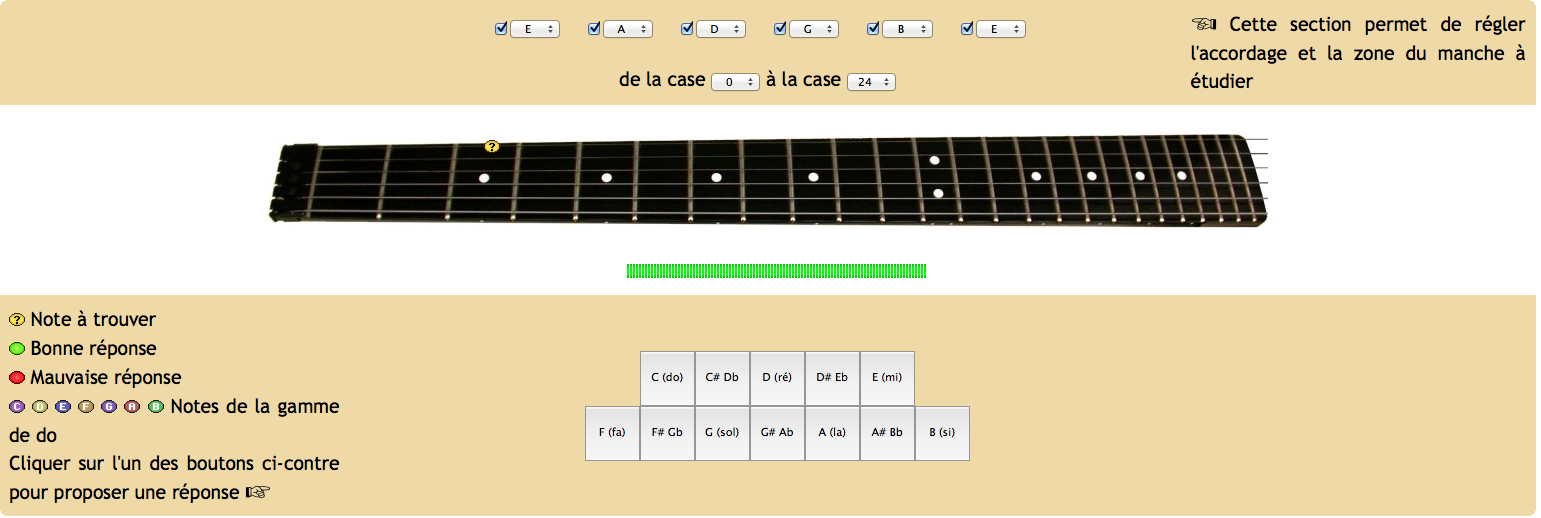
\includegraphics[width=8cm]{images/balezator_manche.png}
			\end{center}
			\begin{itemize}
				\item Jeu de devinettes pour apprendre la position des notes sur le manche
				\item Barre de score pour montrer la progression
			\end{itemize}
	\end{frame} 

	% *** iBalezator ***
	\subsection{iBalezator}
	\begin{frame}

		\frametitle{iBalezator}
		\begin{itemize}
			\item Adaptation du Balezator en ligne pour petits terminaux iOS 8.1
			\item Application dédiée aux guitaristes débutants
			\item Deux modes de jeu :
		\end{itemize}


		\begin{columns}

			 \begin{column}{0.5\textwidth}
				\begin{figure}
					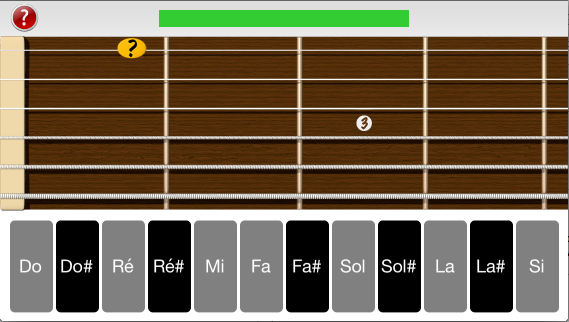
\includegraphics[width=5cm]{images/clavier_question.png}
				\end{figure}

			\end{column}

			 \begin{column}{0.5\textwidth}
				\begin{figure}
					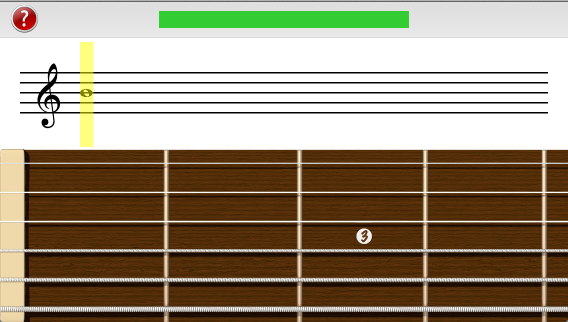
\includegraphics[width=5cm]{images/portee_first_question.png}
					
				\end{figure}
				
			\end{column}

		\end{columns} 
	\end{frame} 


% ******************* Le produit *******************
\section{Le produit}

	\subsection{Mode manche/clavier}
		\begin{frame}
			\frametitle{Mode manche/clavier}

			\begin{minipage}{0.35\linewidth}
				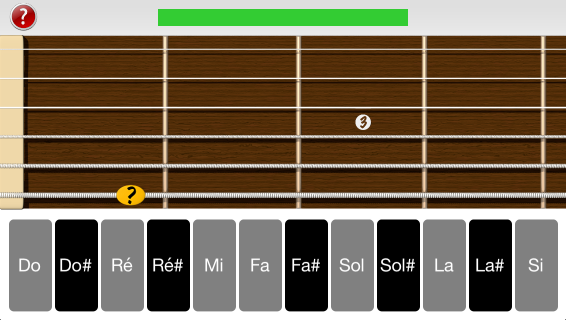
\includegraphics[width=4cm]{images/clavier_question2.png}
			\end{minipage}\hfill
			\begin{minipage}{0.6\linewidth}
				
				\begin{itemize}
					\item Le jeu démarre en mode manche/clavier
					\item Tirage aléatoire d'une note
					\item Affichage du marqueur de question
					\item Son correspondant à la question émis
				\end{itemize}
			\end{minipage}
			\bigbreak
			\pause
			\begin{minipage}{0.35\linewidth}
				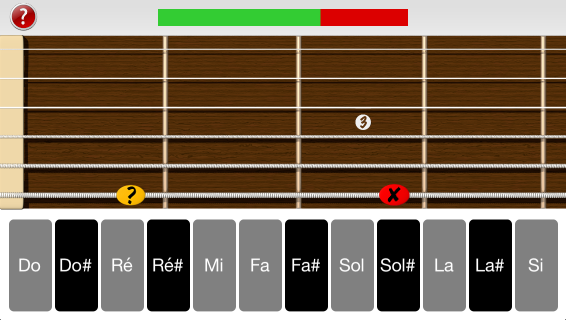
\includegraphics[width=4cm]{images/clavier_bad_answer.png}
			\end{minipage}\hfill
			\begin{minipage}{0.6\linewidth}
				\begin{itemize}
					\item Détection d'une mauvaise réponse
					\item Affichage de la fausse note sur le manche
					\item Son de la fausse note émis
					\item Score mis à jour
				\end{itemize}
			\end{minipage}
			
		\end{frame}	

		\begin{frame}
			\frametitle{Mode manche/clavier}


			\begin{minipage}{0.35\linewidth}
				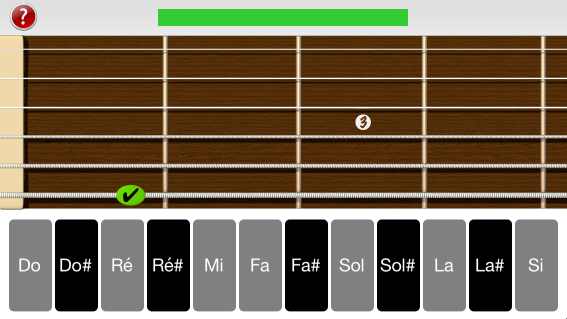
\includegraphics[width=4cm]{images/clavier_good_answer2.png}
			\end{minipage}\hfill
			\begin{minipage}{0.6\linewidth}
				
				\begin{itemize}
					\item Détection d'une bonne réponse
					\item Affichage du marqueur de bonne réponse pendant un certain temps
					\item Son de la note émis
					\item Score mis à jour
				\end{itemize}
			\end{minipage}
			\bigbreak
			\pause
			\begin{minipage}{0.35\linewidth}
				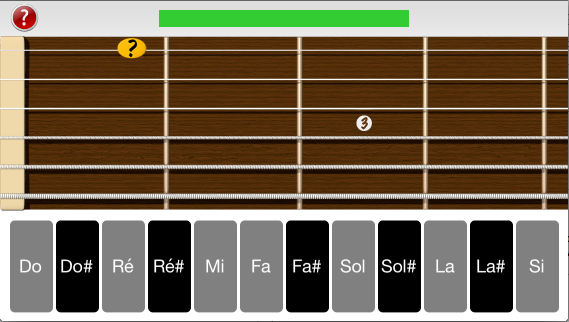
\includegraphics[width=4cm]{images/clavier_question.png}
			\end{minipage}\hfill
			\begin{minipage}{0.6\linewidth}
				
				\begin{itemize}
					\item Génération d'une nouvelle note aléatoire
					\item Son correspondant à la question émis 
					\item Le jeu continue
				\end{itemize}
			\end{minipage}


			\bigbreak

		\end{frame}	

	\subsection{Mode portée/manche}
		\begin{frame}
			\frametitle{Mode portée/manche}

			\begin{minipage}{0.35\linewidth}
				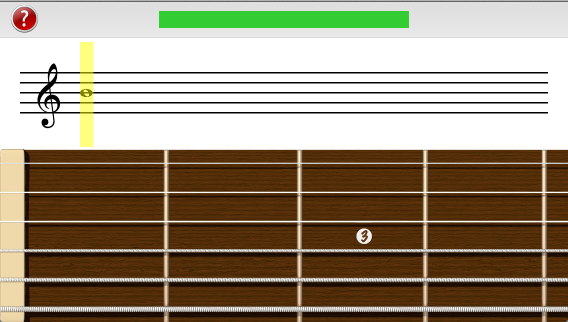
\includegraphics[width=4cm]{images/portee_first_question.png}
			\end{minipage}\hfill
			\begin{minipage}{0.6\linewidth}
				
				\begin{itemize}
					\item Changement de mode : glissé vertical
					\item Génération de notes aléatoires
					\item Affichage sur la portée
					\item Son correspondant à la question émis
				\end{itemize}
			\end{minipage}
			\bigbreak
			\pause
			\begin{minipage}{0.35\linewidth}
				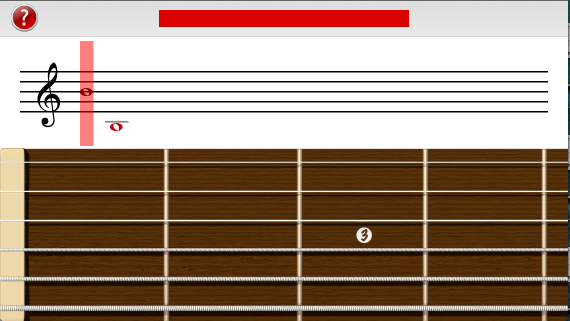
\includegraphics[width=4cm]{images/portee_bad_answer.png}
			\end{minipage}\hfill
			\begin{minipage}{0.6\linewidth}
				
				\begin{itemize}
					\item Détection d'une mauvaise réponse
					\item Affichage sur la portée : surbrillance rouge
					\item Son de la fausse note émis
					\item Score mis à jour
				\end{itemize}
			\end{minipage}
		\end{frame}	

		\begin{frame}
		 \frametitle{Mode portée/manche}
                         
                         \begin{minipage}{0.35\linewidth}
                                 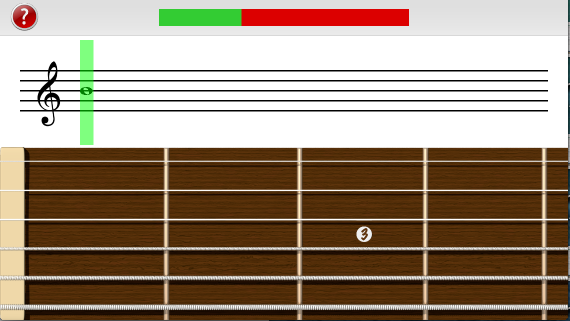
\includegraphics[width=4cm]{images/portee_good_answer.png}
                         \end{minipage}\hfill
                         \begin{minipage}{0.6\linewidth}
 
                                 \begin{itemize}
                                         \item Détection d'une bonne réponse
                                         \item Surbrillance verte pendant un certain temps
                                         \item Son de la bonne note émis
                                         \item Score mis à jour
                                 \end{itemize}
                         \end{minipage}
                         \bigbreak
			\pause
                         \begin{minipage}{0.35\linewidth}
                                 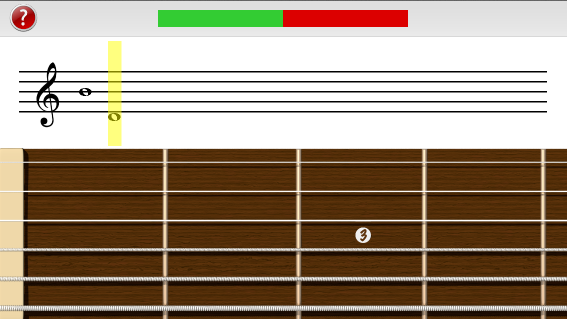
\includegraphics[width=4cm]{images/portee_question2.png}
                         \end{minipage}\hfill
                         \begin{minipage}{0.6\linewidth}
 
                                 \begin{itemize}
                                         \item Question suivante
                                         \item Surbrillance jaune
                                         \item Son de la note en question émis
                                 \end{itemize}
                         \end{minipage}
                 \end{frame}

		\begin{frame}
		 \frametitle{Mode portée/manche}
                         
                         
                         \begin{minipage}{0.35\linewidth}
                                 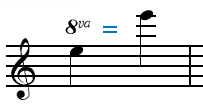
\includegraphics[width=4cm]{images/octava.png}
                         \end{minipage}\hfill
                         \begin{minipage}{0.6\linewidth}
 
                                 \begin{itemize}
					 \item Lignes ajoutées en dehors de la portée pour les notes trop graves ou trop aiguës
                                         \item Notes très aiguës : affichage d'une notation 8va (octava)
                                 \end{itemize}
                         \end{minipage}
\bigbreak
                         \begin{minipage}{0.35\linewidth}
                                 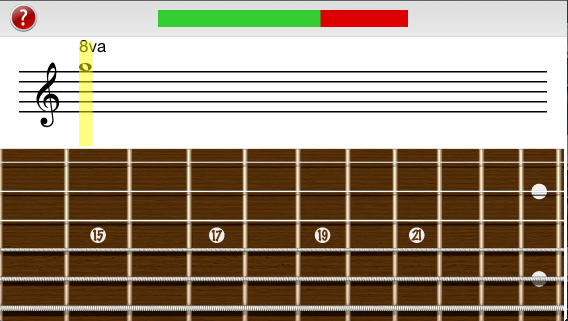
\includegraphics[width=4cm]{images/portee_octava.png}
                         \end{minipage}\hfill
                         \begin{minipage}{0.6\linewidth}
 
                                 \begin{itemize}
                                         \item Notes affichées une octave plus bas à partir de l'octava
                                 \end{itemize}
                         \end{minipage}
		\end{frame}
	
\section{Interface graphique}

	\subsection{Afficher un manche}
		\begin{frame}
		\frametitle{Afficher un manche}
			\begin{itemize}
				\item Une simple image 
				\item Retrouver la correspondance du tap
				\item Quelle est la partie visible
				\item Plusieurs positions pour une même note
			\end{itemize}
			\only<1>{
				\begin{center}
				   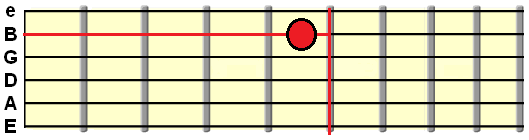
\includegraphics[height=0.2\textheight,keepaspectratio]{images/implementation/correspondance.png}
				\end{center}
			}

			\only<2>{
				\begin{center}
				   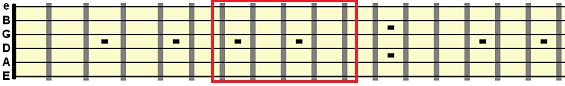
\includegraphics[height=0.2\textheight,keepaspectratio]{images/implementation/partie_visible.png}
				\end{center}
			}

			\only<3>{
				\begin{center}
				   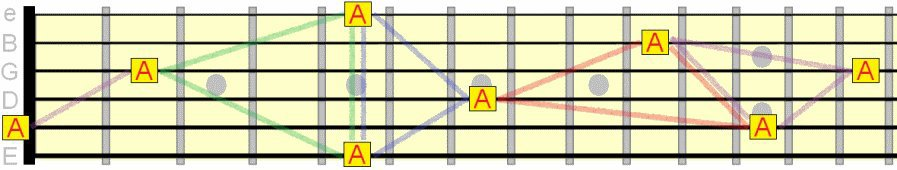
\includegraphics[height=0.2\textheight,keepaspectratio]{images/implementation/notes_enharmoniques.jpg}
				\end{center}
			}
		\end{frame}

	\subsection{Afficher une portée}
		\begin{frame}

		\frametitle{Afficher une portée}
			\begin{itemize}
				\item Dessin de la portée grâce à iOS
				\item Pas de stockage d'image
				\item Dessin vectoriel, traits nets
				\item Adapter le dessin au terminal
				\item Correspondance d'une note du manche sur la portée
			\end{itemize}
			\only<1>{
				\begin{center}
				   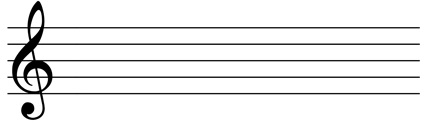
\includegraphics[height=0.2\textheight,keepaspectratio]{images/implementation/cle_sol.jpg}
				\end{center}
			}
			\only<2>{
				\begin{center}
				   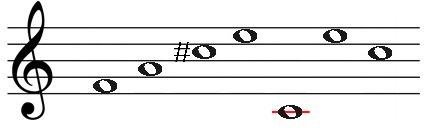
\includegraphics[height=0.2\textheight,keepaspectratio]{images/implementation/staff_implem2v2.jpg}
				\end{center}
			}
			\only<3>{
				\begin{center}
				   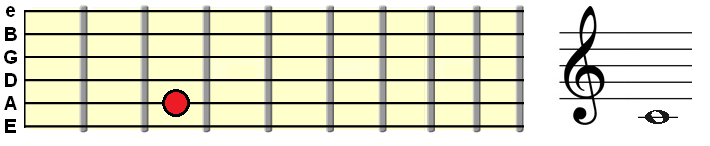
\includegraphics[height=0.2\textheight,keepaspectratio]{images/implementation/portee_manche.png}
				\end{center}
			}	
		\end{frame}

	\section{Génération de son}
		\begin{frame}

		\frametitle{Génération de son}
			\begin{itemize}
				\item Ne pas stocker un fichier audio par note 
				\item AudioKit : génération à partir d'une fréquence
				\item Plusieurs simulations d'instrument
				\item Interface entre notre application et AudioKit 
				\item Jeunesse de la bibliothèque, manque de documentation
			\end{itemize}
		\end{frame}
\section{Conclusion}
		\begin{frame}
		\frametitle{Conclusion}
			Implémentation :
			\begin{itemize}
			\item Difficultés liées au solfège
			\item Swift : ses particularités, implémenter le MVC
			\item Peu de documentation pour la bibliothèque audio
			\end{itemize}
			\pause
			Produit final :
			\begin{itemize}
			\item Mode Clavier/Manche conforme
			\item Mode Portée/Manche fonctionnel
			\item Bibliothèque audio intégrée
			\end{itemize}
			\pause

			Vie future de l'application :
			\begin{itemize}
				\item Mode Basse, gaucher
				\item Choix de l'accordage 
				\item Améliorer les réglages du son
				\item Persistance des données
			\end{itemize}
		\end{frame}
\end{document}
